\label{chapter:Resultados}

\section{Classificação}

\par
\textcolor{red}{Os resultados obtidos com o algoritmo de classificação apresentam um valor mediano de acurácia para o modelo utilizado. A técnica de classificação que foi utilizada, classificou corretamente em torno de 53\% das instâncias que pertence ao conjunto de teste, em relação à classe do resultado que foi obtido. Com base do modelo de árvore de decisão deduzido pelo algoritmo J48, foi possível analisar o grau de interação e a relação das variáveis de acordo com o caminho de interações percorrido pelas respostas do questionário feitas pelos candidatos.}

\par
\textcolor{red}{A árvore obtida apresentou como variável independente principal para a classificação o atributo Deficiencia, que se divide em 5 valores: Nao, Sim visual, Sim outro tipo, Sim fisica e Sim auditiva. As próximas variáveis com maior relevância mudavam de acordo com o valor que era obtido, sendo que, quando a resposta do candidato era de que ele não possuía alguma deficiência ou que ele possuía uma deficiência visual, a variável com maior importância para onde os valores eram direcionados era se ele frequentava ou frequenta cursinho particular, enquanto, para aqueles que possuíam deficiência física ou auditiva eram direcionados para a variável Cor (cor de pele), como apresentada na Figura XX.}

\par
\begin{figure}[!htp]
	\begin{center}
    \caption{\label{fig:waveform_fig} Representação das principais variáveis da árvore de decisão.}
	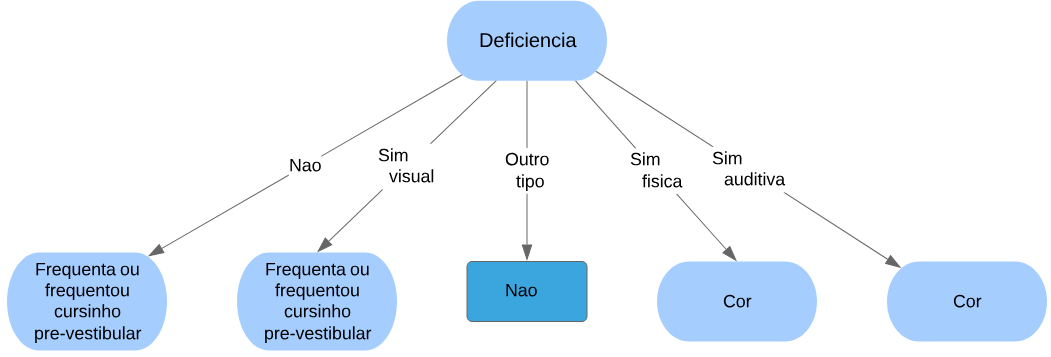
\includegraphics[scale=0.57]{Figuras/Arvore_gerada_grau2.png}
	\end{center}
    \legend{Fonte: Próprio autor.}
\end{figure}


\par
\textcolor{red}{É possível observar na Figura 34, que para os candidatos que responderam que possuíam outro tipo de deficiência, o valor da resposta era direcionado para um nó folha da classe Nao pertencente a variável dependente Aprovado, isto é, os candidatos que possuíam outro tipo de deficiência que não foram mencionados como opção de resposta da questão, não foram capazes de passar no vestibular (um total de 9 candidatos). A partir do terceiro nível de profundidade, para os candidatos que não possuíam nenhum tipo de deficiência a ramificação da árvore se expandia (tracejado pela linha vermelha), enquanto, diferentemente para os candidatos que possuíam algum tipo de deficiência, eles eram direcionados para os nós folhas da variável Aprovado (tracejado pela linha verde), como apresentado na Figura XX.}

\par
\begin{figure}[!htp]
	\begin{center}
    \caption{\label{fig:waveform_fig} Árvore completa.}
	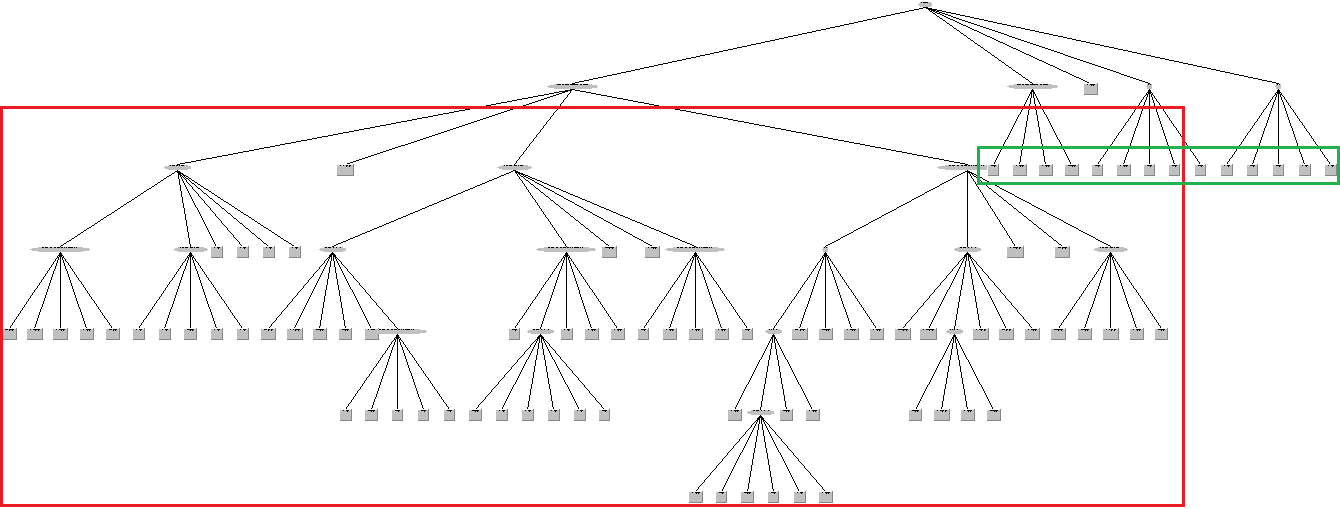
\includegraphics[scale=0.45]{Figuras/Arvore_completa.png}
	\end{center}
    \legend{Fonte: Próprio autor.}
\end{figure}


\subsection{Resultados obtidos para os candidatos que não possuiam nenhum tipo de deficiência}


\par
\textcolor{red}{Avaliando a árvore que foi gerada, através da maior quantidade de registros que se encaixam pelo caminho percorrido das ramificações até as folhas, foi obtido os seguintes resultados, começando pela ramificação maior que era a dos candidatos que não possuiam nenhum tipo de deficiencia, a variavel com maior relevancia que foi classificada após o variavel independente principal era se o candidato frequentava um cursinho pré-vestibular. Foi classificado que todos aqueles que frequentaram por mais de um ano algum cursinho, não foram aprovados no vestibular.}

\par
\textcolor{red}{Para aqueles que frequentaram o cursinho por um ano, o atributo correspondente seguinte era a quantidade de pessoas que moravam com ele, sendo que, a maior taxa de candidatos aprovados para essa variavel era quando possuia 3 pessoas morando com ele e para reprovados era quando possuia de 4 a 5 pessoas. Já para os candidatos que ficavam por um semestre fazendo o cursinho, a variavel correspondente seguinte era o meio de transporte que ele utilizava, a maior taxa de aprovados era pra aqueles que usavam o transporte coletivo e para os reprovados eram os outros tipos de transportes não eram mencionados como opção de resposta.}

\par
\textcolor{red}{Para aqueles que não frequentavam algum cursinho pré-vestibular, a variável classificada com maior relevância, seguinte, era a quantidade de pessoas que moravam com o candidato, e dependendo dos valores que eram respondidos para essa variável, os atributos em sequência variavam entre cor de pele, ocupação do pai e meio de transporte utilizado. Foi notado que as maiores taxas de aprovados eram para os candidatos pardos, que moravam de 3 a 5 pessoas e que o pai era servidor público, já para aqueles que não foram aprovados, as maiores taxas eram quando o candidato possuía de quatro ou mais pessoas morando com ele, o pai possuía outro tipo de ocupação e o meio de transporte utilizado era o coletivo.}


\subsection{Resultados obtidos para os candidatos que possuiam algum tipo de deficiência}


\par
\textcolor{red}{}